\documentclass[a4paper,12pt]{report}

\usepackage{cmap}
\usepackage[T2A]{fontenc}
\usepackage[utf8]{inputenc}
\usepackage[english,russian]{babel}
\usepackage{listings}
\usepackage{amsmath}
\usepackage{float}
\usepackage{csquotes}
\usepackage{mathtools}

\usepackage{xcolor}
\usepackage{hyperref}

\usepackage{graphicx}
\graphicspath{ {./img/} }

\definecolor{dkgreen}{rgb}{0,0.6,0}
\definecolor{gray}{rgb}{0.5,0.5,0.5}
\definecolor{mauve}{rgb}{0.58,0,0.82}

\lstset{
    language=Python,                
    basicstyle=\small\sffamily, 
    numbers=left,               
    numberstyle=\tiny,           
    stepnumber=1,                   
    numbersep=5pt,                
    aboveskip=3mm,
    belowskip=3mm,
    showstringspaces=false,
    columns=flexible,
    captionpos=b, 
    basicstyle={\small\ttfamily},
    numbers=left,
    numberstyle=\tiny\color{gray},
    keywordstyle=\color{blue},
    commentstyle=\color{mauve},
    stringstyle=\color{dkgreen},
    breaklines=true,
    breakatwhitespace=true,
    tabsize=3
}

\title{Лабораторная работа №12\\GNU Radio}
\author{Крынский Павел}
\date{\today}

\begin{document}

\maketitle
\tableofcontents
\listoffigures

\maketitle

\chapter{Основная часть}
\section{Передача сигнала}
 
 
Первым этапов является передача QPSK сигнала. Нам нужно сгенерировать поток битов и смоделировать его в созвездие. Для этого используем блок Constellation Modulator, который использует объект Constellation. 

Объект Constellation позволяет нам определить, как символы кодируются. Constellation Modulator ожидает упакованные байты, поэтому у нас есть генератор случайных источников, предоставляющий байты со значениями 0 - 255. 

Мы хотим, чтобы количество выборок на символ было как можно меньше (минимальное значение - 2). Здесь мы будем использовать 4, что больше, чем нам нужно, но полезно для визуализации сигнала в разных областях. 

Теперь мы устанавливаем значение избыточной пропускной способности. Модулятор созвездия использует RRC (root raised cosine) фильтр, который дает нам один параметр для настройки коэффициента спада фильтра. Следующий рисунок показыeт различные значения избыточной полосы пропускания. Типичные значения находятся в диапазоне от 0,2 до 0,35: 

\begin{figure}[H]
        \centering
        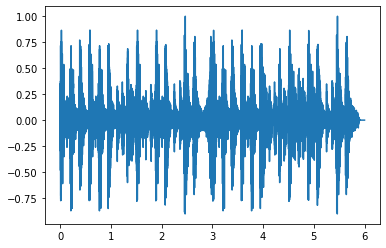
\includegraphics[width=0.75\textwidth]{1.png}
        \caption{Получившийся сигнал}
        \label{fig:ig4_1}
\end{figure}

Следующий пример отображает как передаваемый сигнал, так и часть цепочки приемника во времени и частоте, а также график созвездия.

\begin{figure}[H]
        \centering
        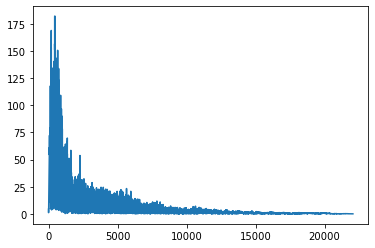
\includegraphics[width=0.75\textwidth]{2.png}
        \caption{Пример с QPSK Constellation}
        \label{fig:ig4_1}
\end{figure}

\begin{figure}[H]
        \centering
        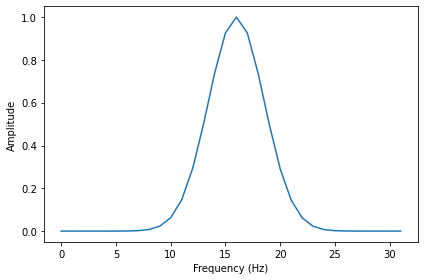
\includegraphics[width=0.75\textwidth]{3.png}
        \caption{Временной, фазовый и частотный графики}
        \label{fig:ig4_1}
\end{figure}

На графике созвездия видны эффекты повышения частоты дискретизации и фильтрации. Фильтр RRC добавляет преднамеренные собственные помехи, известные как межсимвольные помехи (ISI). 

Частотный график показывает сигнал с хорошей формой, который скатывается в шум. Если бы мы не установили формирующий фильтр на сигнал, мы бы передавали прямоугольные волны, которые производят много энергии в соседних каналах. Благодаря уменьшению внеполосных излучений наш сигнал теперь остается в пределах полосы пропускания нашего канала. 

\section{Добавление канала}

В первом пункте мы рассмотрели только механизм передачи QPSK сигнала. Теперь рассмотрим эффекты канала и то, как сигнал искажается между тем, когда он был передан, и тем, когда мы получаем его на приемнике. Первым шагом будет добавление модели канала. Для начала используем самый базовый блок Channel Model в GNU Radio. 

Этот блок позволяет нам смоделировать несколько основных проблем, с которыми нам приходится иметь дело. Первая проблема с приемниками - шум. Тепловой шум в приемнике вызывает шум, который мы называем аддитивным белым гауссовым шумом (AWGN). Мы устанавливаем мощность шума, регулируя значение шумового напряжения модели канала. Здесь мы указываем напряжение вместо мощности, потому что нам нужно знать полосу пропускания сигнала, чтобы правильно рассчитать мощность.

Другая существенная проблема между двумя радиостанциями - это разные тактовые сигналы, управляющие частотой радиостанций. Тактовые сигналы несовершенны, и, следовательно, отличаются между радиостанциями. Одно радио передает номинально на fc (скажем, 450 МГц), но действительно оно передает на fc + fdelta1. Между тем, другая радиостанция имеет другой тактовый сигнал и, следовательно, другое смещение, fdelta2. В конце концов, полученный сигнал будет на fdelta1 + fdelta2 от того, где мы думаем, что он должен быть. 

C проблемой тактовых сигналов связана проблема идеальной точки выборки. Мы увеличили частоту дискретизации нашего сигнала в передатчике, но при его получении нам необходимо произвести выборку сигнала в исходной точке выборки, чтобы максимизировать мощность сигнала и минимизировать межсимвольные помехи. После добавления второго фильтра RRC, мы можем видеть, что среди 4 выборок на символ одна из них находится в идеальной точке выборки. Но, опять же, две радиостанции работают на разных скоростях, поэтому идеальная точка выборки неизвестна. 

\begin{figure}[H]
        \centering
        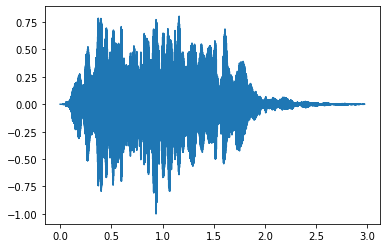
\includegraphics[width=0.75\textwidth]{4.png}
        \caption{Графики с шумом и сдвигами}
        \label{fig:ig4_1}
\end{figure}

График созвездия показывает нам облако образцов, намного хуже того, с чего мы начали на последнем этапе.

\section{Временное восстановление}

Теперь нужно восстановить исходный сигнал из полученного искажённого сигнала. Есть много алгоритмов, которые мы могли бы использовать для нивелирования каждого из негативных эффектов. Некоторые могут осуществлять совместное восстановление от нескольких эффектов одновременно. Мы будем использовать алгоритм восстановления многофазных часов. 

Начнем с временного восстановления. Сначала нужно найти наилучшее время для выборки входящих сигналов, что позволит максимально увеличить отношение сигнала к шуму (SNR) каждой выборки, а также уменьшить влияние межсимвольных помех (ISI). 

Мы можем проиллюстрировать проблему ISI, используя пример, где мы создаем четыре отдельных символа единицы и затем фильтруем их. На первом этапе фильтрации выполняется повышение частоты дискретизации до 'sps’ выборок на символ и используется RRC фильтр. Затем применяется ещё один RRC фильтр. Сворачивая два RRC фильтра вместе, мы получаем RC фильтр, который является формой фильтра Найквиста. 

Графики, приведённые ниже, показывают различия между RRC- и RC-фильтрованными символами. Без фильтрации Найквиста в идеальной точке выборки каждого символа другие символы имеют некоторую энергию. Если мы сложим эти символы вместе, что мы и сделаем, имея непрерывный поток выборок, энергия других символов исказит символ в данной точке. Но в RC-фильтрованном выходе энергия других символов равна 0 в идеальной точке выборки для данного символа во времени. Это означает, что, если мы производим выборку в идеальной точке выборки, мы получаем энергию только от текущего символа без помех от других символов в потоке. 

\begin{figure}[H]
        \centering
        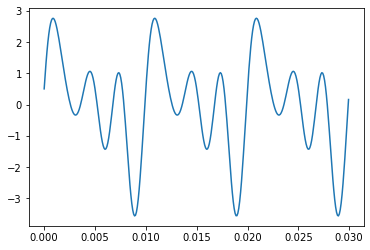
\includegraphics[width=0.75\textwidth]{5.png}
        \caption{Сравнение RRC и RC фильтров}
        \label{fig:ig4_1}
\end{figure}

Теперь давайте посмотрим, что происходит из-за различий в тактовых сигналах между передатчиком и приёмником и как это влияет на точки выборки. Тактовые сигналы несовершенны, и поэтому они а) начинаются в разные моменты времени и б) дрейфуют относительно друг друга. Мы моделируем это, добавляя ресемплер, который немного настраивает время выборки символа между передаваемым сигналом и приемником. Разница тактовых сигналов, показанная здесь, в 1.125, является очень большой, это сделано для визуализации. На самом деле, временные различия находятся в пределах миллионных долей. Заметим, что при таких выборках, собираемых в разные моменты времени, идеальный период выборки неизвестен, и любая сделанная выборка также будет включать ISI. 

\begin{figure}[H]
        \centering
        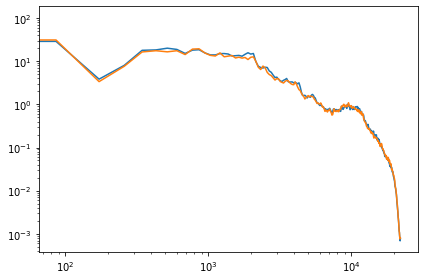
\includegraphics[width=0.75\textwidth]{6.png}
        \caption{Пример подобного тактирования}
        \label{fig:ig4_1}
\end{figure}

\section{Подробная информация о Polyphase Clock Sync}

Существуют различные алгоритмы, которые мы можем использовать для восстановления тактового сигнала на приемнике, и почти все они включают в себя некоторый цикл управления с обратной связью. Те, которые не включают, обычно используют некоторое известное слово. Мы будем использовать метод ‘polyphase filterbank clock recovery”. Этот метод позволяет сделать сразу 3 вещи. Во-первых, он выполняет временное восстановление. Во-вторых, он согласовывает фильтр приемника и, тем самым, устраняет ISI. В-третьих, он понижает дискретизацию сигнала и производит выборки с частотой 1 sps. 

Блок синхронизации многофазных часов работает, вычисляя первую производную входящего сигнала, которая связана с тактовым смещением сигнала. Рассмотрим работу блока на примерах. В примере мы можем видеть, как идеально всё выглядит, когда нет смещения тактовой частоты. Точка выборки, которая нам нужна, очевидно, находится на 0,25 мс. Дифференциальный фильтр ([-1, 0, 1]) генерирует дифференциал символа, и, как показано на следующем рисунке, результат этого фильтра в правильной точке выборки равен 0. Мы можем проинвертировать этот оператор и вместо этого сказать, что если на выходе дифференциального фильтра 0, то мы нашли оптимальную точку выборки.

\begin{figure}[H]
        \centering
        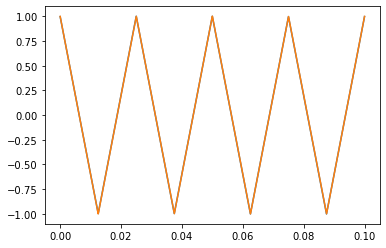
\includegraphics[width=0.75\textwidth]{7.png}
        \caption{Delay = 0}
        \label{fig:ig4_1}
\end{figure}

\begin{figure}[H]
        \centering
        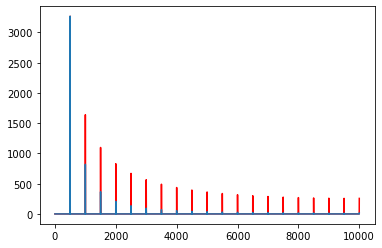
\includegraphics[width=0.75\textwidth]{8.png}
        \caption{Delay = 1}
        \label{fig:ig4_1}
\end{figure}

Вместо того, чтобы использовать один фильтр, мы можем создать серию фильтров, каждый из которых будет иметь свою фазу. И если у нас будет достаточно фильтров с разными фазами, одна из них окажется правильной и даст нам желаемое значение. Рассмотрим симуляцию, которая строит 5 фильтров, что означает 5 различных фаз.

\begin{figure}[H]
        \centering
        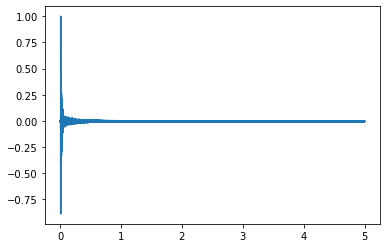
\includegraphics[width=0.75\textwidth]{9.png}
        \caption{График схемы с несколькими фильтрами}
        \label{fig:ig4_1}
\end{figure}

Видно, что сигнал, помеченный как d (sym0) / dt + phi3 в правильной точке выборки равен 0. Это говорит о том, что наша идеальная точка выборки возникает при этом сдвиге фазы. Поэтому, если мы возьмем фильтр RRC нашего приемника и настроим его фазу на phi3 (которая равна 3 * 2pi / 5), то мы сможем исправить несоответствие синхронизации и выбрать идеальную точку выборки. 

Но это лишь моделируемое приближение, в действительности выборки каждого фильтра не будут происходить в один и тот же момент времени. Чтобы действительно увидеть такое поведение, мы должны увеличить частоту дискретизации в количество раз, равное количеству фильтров. Мы можем рассматривать эти разные фильтры как части одного большого фильтра с частотой дискретизации в M раз больше, где M = 5 в нашем простом примере. Мы могли бы увеличить частоту нашего входящего сигнала и выбрать момент времени, когда мы получаем 0 на выходе фильтра, но проблема в том, что мы говорим о большой сложности вычислений, поскольку она пропорциональна нашей частоте дискретизации. Вместо этого, будем работаем с фильтрами с разными фазами на входящей частоте дискретизации, но, имея такой набор фильтров, мы сможем получить эффект от работы с фильтром с увеличенной частотой дискретизации без дополнительных вычислительных затрат. 

Таким образом, в примере выше мы сместили частоту дискретизации на некоторый известный коэффициент 1,2 и обнаружили, что можем использовать один из пяти фильтров в качестве идеальной точки выборки. К сожалению, у нас действительно есть только 5 различных фаз, которые мы можем точно исправить. Любое смещение выборки между этими фазами все равно приведет к неправильной выборке с добавлением ISI. Поэтому в алгоритме восстановления тактовой частоты мы используем большее количество фильтров. Не углубляясь в математику, мы можем использовать 32 фильтра, чтобы максимальный шум от ISI был меньше шума квантования 16-битного значения. Если нам нужна точность более 16 бит, мы можем использовать больше фильтров. 

В итоге у нас есть большой банк фильтров, один из которых находится очень близко к идеальному смещению фазы дискретизации. Как мы автоматически выберем нужный фильтр? Используя цикл управления 2-го порядка (2nd order control loop), как мы почти всегда делаем в ситуациях восстановления. Сигналом ошибки восстановления будет являться выход дифференциального фильтра. Цикл управления запускается на одном из фильтров и вычисляет выходной сигнал как сигнал ошибки. Затем он перемещается вверх или вниз по банку фильтров в зависимости от полученного сигнала ошибки и пытается найти, где сигнал ошибки наиболее близок к нулю, тем самым находя оптимальный фильтр. 

\section{Использование Polyphase Clock Sync в приёмнике}

Применим рассмотренный блок в нашей симуляции. Пример берет выходные данные модели канала и пропускает их через блок синхронизации. Сам блок использует 32 фильтра по причинам, которые мы обсуждали ранее и принимает на вход число ожидаемых выборок на символ, но это число - всего лишь наше предположение, внутри блок будет адаптировать его, основываясь на скоростях входящего сигнала. Заметьте, однако, что мы настроили эту симуляцию так, что оценка немного отличается от 4-х sps, которые мы передаем. Это делается для имитации начального тактового смещения между передатчиком и приемником. 

\begin{figure}[H]
        \centering
        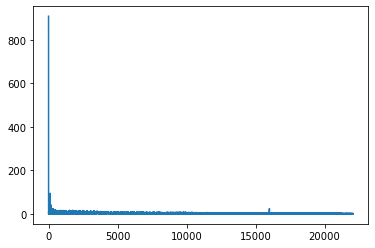
\includegraphics[width=0.75\textwidth]{10.png}
        \caption{График схемы с несколькими фильтрами}
        \label{fig:ig4_1}
\end{figure}

При запуске этого скрипта мы видим созвездие слева как полученный сигнал
до восстановления синхронизации и справа после восстановления синхронизации. Это все еще немного шумно из-за ISI после 32 фильтров, который быстро поглощается шумом, когда мы устанавливаем значение параметра Noise Voltage больше 0.

\section{Многолучевое распространение}

Сначала узнаем, что такое многолучевое распространение, откуда оно берется и как оно влияет на наши коммуникационные возможности. 

Многолучевое распространение обусловлено тем, что в большинстве сред связи у нас нет единого пути прохождения сигнала от передатчика к приемнику. Как показано на рисунке ниже, каждый раз, когда появляется объект, отражающий сигнал, между двумя узлами может быть установлен новый путь. Поверхности, такие как здания, знаки, деревья, люди, кошки и т.д. могут создавать отражения сигналов. Сигнал, проходя по каждому из путей, будет доходить до приемника за разное время, в зависимости от длины пути.  

\begin{figure}[H]
        \centering
        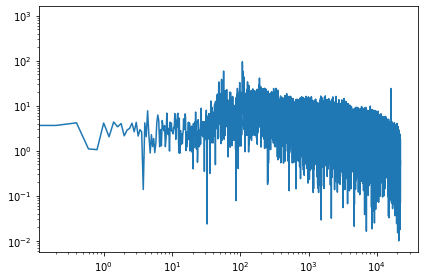
\includegraphics[width=0.75\textwidth]{11.png}
        \caption{График схемы с несколькими фильтрами}
        \label{fig:ig4_1}
\end{figure}

Воздействие комбинации этих сигналов на приемник - искажение сигнала.
Если разница во времени между отражениями достаточно мала по сравнению с
шириной символа, искажение может быть внутри символа - внутрисимвольная
интерференция. Если время отражения превышает время символа, отражение
от одного символа будет влиять на следующие сигналы - еще одна причина
межсимвольной интерференции.

Нам нужно исправить это поведение, и мы можем сделать это, используя механизм, очень похожий на стереоэквалайзер. Фактически мы называем их эквалайзерами. С помощью стереофонического эквалайзера мы можем изменить усиление определенных частот, чтобы либо подавить, либо усилить эти сигналы,
наиболее распространенными из которых являются низкие и высокие частоты.

Это моделирование настраивает модель канала, чтобы предоставить каналу
пять элементов управления эквалайзером, четыре из которых мы можем изменить. Эти элементы управления настроены одинаково по частоте, и мы можем настроить их от 0 до 1. При значении 1 элемент управления позволит этим частотам проходить без помех. При значении 0 они будут производить глубокий нуль в спектре, который повлияет на все частоты вокруг него. График частоты установлен на среднее значение.

Хотя в этом примере мы явно контролируем частотную область, на самом деле мы играем с возможностью создать эквалайзер, который может корректировать или регулировать частотную характеристику принятого сигнала. В конечном итоге цель показана на рисунке ниже, где многолучевой канал создает некоторые искажения в сигнале, как показано в частотной области. Задача эквалайзера - инвертировать этот канал. По сути, мы хотим отменить искажение, вызванное каналом, чтобы выходной сигнал эквалайзера был ровным. Но вместо того, чтобы настраивать краны вручную, у нас есть алгоритмы, которые обновляют эти краны за нас. Наша задача - использовать правильный алгоритм эквалайзера и настроить параметры. Одним из важных параметров здесь является количество нажатий в эквалайзере. Как мы видим в нашем моделировании, пять нажатий дают довольно грубый контроль над частотной характеристикой. В качестве альтернативы, чем больше ответвлений, тем больше времени требуется как на вычисление ответвлений, так и на запуск эквалайзера против сигнала.


\begin{figure}[H]
        \centering
        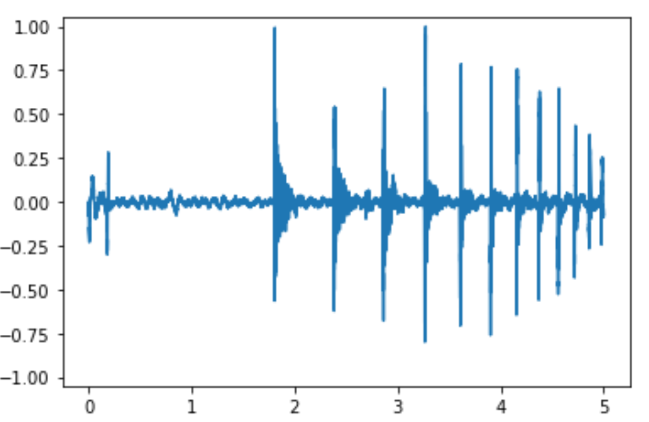
\includegraphics[width=0.75\textwidth]{12.png}
        \caption{Сравнение принятого сигнала с изначальным AWGN (аддитивный белый гауссовский шум)}
        \label{fig:ig4_1}
\end{figure}

\section{Эквалайзеры}

GNU Radio поставляется с двумя легко используемыми эквалайзерами, CMA и DD LMS. Мы будем использовать DD LMS (Decision-Directed Least Mean Squared). 

CMA и DD LMS довольно похожи в плане параметров, за исключением одной важной особенности. DD LMS, в отличие от CMA – не слепой эквалайзер, он требует информации о принимаемом сигнале. Ему необходимо знать точки созвездия. 

Этот эквалайзер отлично подходит для сигналов, которые не соответствуют требованию постоянного модуля алгоритма CMA. С другой стороны, если SNR достаточно плох, принимаемые решения будут неправильными, что может ухудшить производительность приемника. Кроме того, DD LMS более сложен в вычислительном отношении. Однако, когда у нас есть сигнал хорошего качества, этот эквалайзер может генерировать более высококачественные сигналы, нежели CMA, поскольку у него есть информация о сигнале. 

\begin{figure}[H]
        \centering
        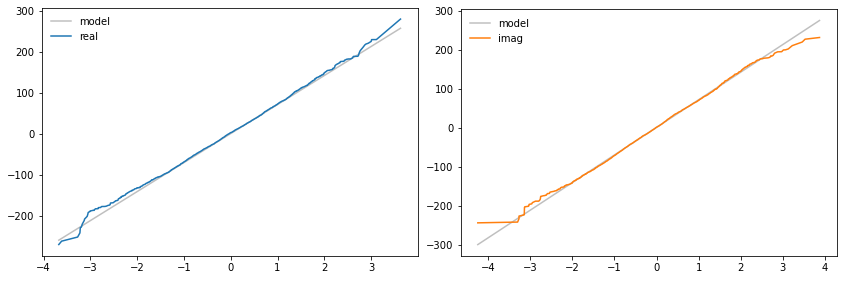
\includegraphics[width=0.75\textwidth]{13.png}
        \caption{Сравнение многолучевого сигнала до и после эквалайзера}
        \label{fig:ig4_1}
\end{figure}

\section{Фазовая частотная коррекция }

У нас все ещё остаётся проблема сдвига фазы и частоты. Эквалайзеры, как правило, не адаптируются быстро, поэтому смещение частоты может легко превысить их возможности. 

Две вещи об этом этапе. Во-первых, мы будем использовать цикл второго порядка, чтобы мы могли отслеживать как фазу, так и частоту, которая является производной фазы по времени. Во-вторых, тип восстановления, с которым мы здесь будем иметь дело, предполагает, что мы делаем точную коррекцию частоты. Поэтому мы должны быть уверены, что мы уже находимся достаточно близко к идеальной частоте. 

Мы будем использовать цикл Костаса.Блок Costas Loop может синхронизировать BPSK, QPSK и 8PSK. 

Этот блок использует цикл второго порядка и поэтому определяется параметром пропускной способности цикла. Другая вещь, которая ему необходима - это порядок модуляции PSK (2 для BPSK, 4 для QPSK и 8 для 8PSK). На следующем рисунке мы установили шум, тактовое смещение, простой многолучевой канал и смещение частоты. После эквалайзера мы видим, что все символы находятся на единичной окружности, но вращаются из-за смещения частоты, которое пока не исправляется. На выходе блока Costas Loop мы можем увидеть исходное созвездие, хоть и с дополнительным шумом, с которым мы ничего не можем поделать. 

\begin{figure}[H]
        \centering
        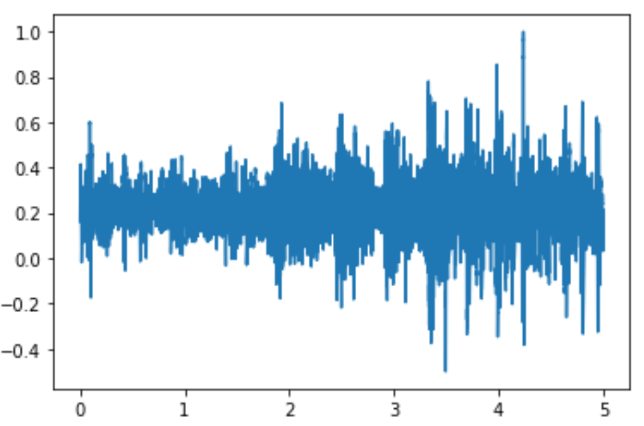
\includegraphics[width=0.75\textwidth]{14.png}
        \caption{}
        \label{fig:ig4_1}
\end{figure}

\section{Декодирование}

Декодируем сигнал. Используя пример диаграммы , мы добавляем квадратурный демодулятор после Costas Loop. На этом этапе мы получаем символы от 0 до 3, потому что это размер нашего алфавита в схеме QPSK. Но из этих 0-3 символов, как мы можем точно знать, что у нас такое же отображение символов в точках созвездия, которое мы делали при передаче? К счастью, мы избежали этой проблемы, передав дифференциальные символы. На самом деле мы не передавали само созвездие, мы передавали разницу между символами созвездия, установив для параметра «Differential» в блоке «Constellation Modulator» значение «True».  

\begin{figure}[H]
        \centering
        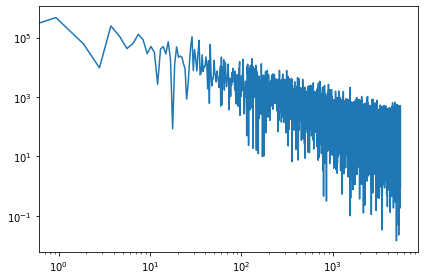
\includegraphics[width=0.75\textwidth]{15.png}
        \caption{}
        \label{fig:ig4_1}
\end{figure}

Блок-схема использует блок “PSK Demod” для преобразования дифференциально-кодированных символов обратно в их исходные символы. Но даже отсюда наши символы не совсем верны. Это самая сложная часть демодуляции. На этапах синхронизации физика и математика была на нашей стороне. Теперь, однако, мы должны интерпретировать некоторый символ, основываясь на том, что это сказал кто-то другой. Мы, в основном, просто должны знать это отображение. И, к счастью, мы это делаем, поэтому мы используем блок Map для преобразования символов из дифференциального декодера в исходные. Теперь у нас есть исходные символы от 0 до 3, поэтому давайте распакуем эти 2 бита на символ в биты, используя блок распаковки битов. Теперь у нас есть оригинальный поток данных!  

Остался вопрос: как узнать, что это оригинальный битовый поток? Для этого сравним его с входным потоком битов, что мы можем сделать, т.к. это симуляция, и у нас есть доступ к переданным данным. Передатчик генерировал упакованные биты, поэтому мы снова используем битовый блок распаковки. Затем мы преобразуем эти потоки в значения с плавающей запятой 0,0 и 1,0. Сравнение этих двух потоков непосредственно ничего не покажет. Почему? Из-за того, что цепочка приемника имеет много блоков и фильтров, которые задерживают сигнал, принятый сигнал отстает на некоторое количество битов. Чтобы компенсировать это, мы должны задержать переданный сигнал на ту же величину, используя блок “Delay”.  
\begin{figure}[H]
        \centering
        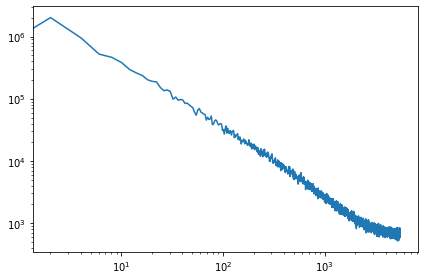
\includegraphics[width=0.75\textwidth]{16.png}
        \caption{Получившийся график с окном Constellation}
        \label{fig:ig4_1}
\end{figure}
 
\begin{figure}[H]
        \centering
        \includegraphics[width=0.75\textwidth]{17.png}
        \caption{Получившийся график с окном Symbols}
        \label{fig:ig4_1}
\end{figure}

\section{Выводы}

В ходе выполнения работы мы познакомились с GNU Radio. Научились генерировать сигналы, добавлять к ним шум, восстанавливать их. Посмотрели работу эквалайзера, Costas Loop и Polyphase Clock Sync.

\end{document}
